%% LyX 2.3.2 created this file.  For more info, see http://www.lyx.org/.
%% Do not edit unless you really know what you are doing.
\documentclass[english,aspectratio=169,handout]{beamer}
\usepackage{mathptmx}
\usepackage{eulervm}
\usepackage[T1]{fontenc}
\usepackage[latin9]{inputenc}
\usepackage{babel}
\usepackage{url}
\usepackage{amsmath}
\usepackage{amssymb}
\usepackage{graphicx}
\usepackage{dsfont}
\ifx\hypersetup\undefined
  \AtBeginDocument{%
    \hypersetup{unicode=true,pdfusetitle,
 bookmarks=true,bookmarksnumbered=false,bookmarksopen=false,
 breaklinks=false,pdfborder={0 0 0},pdfborderstyle={},backref=false,colorlinks=true,
 allcolors=NYUPurple,urlcolor=LightPurple}
  }
\else
  \hypersetup{unicode=true,pdfusetitle,
 bookmarks=true,bookmarksnumbered=false,bookmarksopen=false,
 breaklinks=false,pdfborder={0 0 0},pdfborderstyle={},backref=false,colorlinks=true,
 allcolors=NYUPurple,urlcolor=LightPurple}
\fi

\makeatletter
%%%%%%%%%%%%%%%%%%%%%%%%%%%%%% Textclass specific LaTeX commands.
% this default might be overridden by plain title style
\newcommand\makebeamertitle{\frame{\maketitle}}%
% (ERT) argument for the TOC
\AtBeginDocument{%
  \let\origtableofcontents=\tableofcontents
  \def\tableofcontents{\@ifnextchar[{\origtableofcontents}{\gobbletableofcontents}}
  \def\gobbletableofcontents#1{\origtableofcontents}
}

%%%%%%%%%%%%%%%%%%%%%%%%%%%%%% User specified LaTeX commands.
\usetheme{CambridgeUS} 
\beamertemplatenavigationsymbolsempty


% Set Color ==============================
\definecolor{NYUPurple}{RGB}{87,6,140}
\definecolor{LightPurple}{RGB}{165,11,255}


\setbeamercolor{title}{fg=NYUPurple}
%\setbeamercolor{frametitle}{fg=NYUPurple}
\setbeamercolor{frametitle}{fg=NYUPurple}

\setbeamercolor{background canvas}{fg=NYUPurple, bg=white}
\setbeamercolor{background}{fg=black, bg=NYUPurple}

\setbeamercolor{palette primary}{fg=black, bg=gray!30!white}
\setbeamercolor{palette secondary}{fg=black, bg=gray!20!white}
\setbeamercolor{palette tertiary}{fg=gray!20!white, bg=NYUPurple}

\setbeamertemplate{headline}{}

\setbeamercolor{parttitle}{fg=NYUPurple}
\setbeamercolor{sectiontitle}{fg=NYUPurple}
\setbeamercolor{sectionname}{fg=NYUPurple}
\setbeamercolor{section page}{fg=NYUPurple}

\AtBeginSection[]{
  \begin{frame}
  \vfill
  \centering
\setbeamercolor{section title}{fg=NYUPurple}
 \begin{beamercolorbox}[sep=8pt,center,shadow=true,rounded=true]{title}
    \usebeamerfont{title}\usebeamercolor[fg]{title}\insertsectionhead\par%
  \end{beamercolorbox}
  \vfill
  \end{frame}
}

\makeatother

\begin{document}
\global\long\def\reals{\mathbf{R}}%
 
\global\long\def\integers{\mathbf{Z}}%
 
\global\long\def\naturals{\mathbf{N}}%
 
\global\long\def\rationals{\mathbf{Q}}%
 
\global\long\def\ca{\mathcal{A}}%
 
\global\long\def\cb{\mathcal{B}}%
 
\global\long\def\cc{\mathcal{C}}%
 
\global\long\def\cd{\mathcal{D}}%
 
\global\long\def\ce{\mathcal{E}}%
 
\global\long\def\cf{\mathcal{F}}%
 
\global\long\def\cg{\mathcal{G}}%
 
\global\long\def\ch{\mathcal{H}}%
 
\global\long\def\ci{\mathcal{I}}%
 
\global\long\def\cj{\mathcal{J}}%
 
\global\long\def\ck{\mathcal{K}}%
 
\global\long\def\cl{\mathcal{L}}%
 
\global\long\def\cm{\mathcal{M}}%
 
\global\long\def\cn{\mathcal{N}}%
 
\global\long\def\co{\mathcal{O}}%
 
\global\long\def\cp{\mathcal{P}}%
 
\global\long\def\cq{\mathcal{Q}}%
 
\global\long\def\calr{\mathcal{R}}%
 
\global\long\def\cs{\mathcal{S}}%
 
\global\long\def\ct{\mathcal{T}}%
 
\global\long\def\cu{\mathcal{U}}%
 
\global\long\def\cv{\mathcal{V}}%
 
\global\long\def\cw{\mathcal{W}}%
 
\global\long\def\cx{\mathcal{X}}%
 
\global\long\def\cy{\mathcal{Y}}%
 
\global\long\def\cz{\mathcal{Z}}%
 
\global\long\def\ind#1{1(#1)}%
 %\newcommand{\pr}{P}
\global\long\def\pr{\mathbb{P}}%
 
\global\long\def\predsp{\cy}%
 %{\hat{\cy}}
\global\long\def\outsp{\cy}%

\global\long\def\prxy{P_{\cx\times\cy}}%
 
\global\long\def\prx{P_{\cx}}%
 
\global\long\def\prygivenx{P_{\cy\mid\cx}}%
 %\newcommand{\ex}{E}
\global\long\def\ex{\mathbb{E}}%
 
\global\long\def\var{\textrm{Var}}%
 
\global\long\def\cov{\textrm{Cov}}%
 
\global\long\def\sgn{\textrm{sgn}}%
 
\global\long\def\sign{\textrm{sign}}%
 
\global\long\def\kl{\textrm{KL}}%
 
\global\long\def\law{\mathcal{L}}%
 
\global\long\def\eps{\varepsilon}%
 
\global\long\def\as{\textrm{ a.s.}}%
 
\global\long\def\io{\textrm{ i.o.}}%
 
\global\long\def\ev{\textrm{ ev.}}%
 
\global\long\def\convd{\stackrel{d}{\to}}%
 
\global\long\def\eqd{\stackrel{d}{=}}%
 
\global\long\def\del{\nabla}%
 
\global\long\def\loss{\ell}%
 
\global\long\def\risk{R}%
 
\global\long\def\emprisk{\hat{R}}%
 
\global\long\def\lossfnl{L}%
 
\global\long\def\emplossfnl{\hat{L}}%
 
\global\long\def\empminimizer#1{\hat{#1}^{*}}%
 
\global\long\def\minimizer#1{#1^{*}}%
\global\long\def\optimizer#1{#1^{*}}%
 
\global\long\def\etal{\textrm{et. al.}}%
 
\global\long\def\tr{\operatorname{tr}}%

\global\long\def\trace{\operatorname{trace}}%
 
\global\long\def\diag{\text{diag}}%
 
\global\long\def\rank{\text{rank}}%
 
\global\long\def\linspan{\text{span}}%
 
\global\long\def\spn{\text{span}}%
 
\global\long\def\proj{\text{Proj}}%
 
\global\long\def\argmax{\operatornamewithlimits{arg\, max}}%
 
\global\long\def\argmin{\operatornamewithlimits{arg\, min}}%

\global\long\def\bfx{\mathbf{x}}%
 
\global\long\def\bfy{\mathbf{y}}%
 
\global\long\def\bfl{\mathbf{\lambda}}%
 
\global\long\def\bfm{\mathbf{\mu}}%
 
\global\long\def\calL{\mathcal{L}}%

\global\long\def\vw{\boldsymbol{w}}%
 
\global\long\def\vx{\boldsymbol{x}}%
 
\global\long\def\vxi{\boldsymbol{\xi}}%
 
\global\long\def\valpha{\boldsymbol{\alpha}}%
 
\global\long\def\vbeta{\boldsymbol{\beta}}%
 
\global\long\def\vsigma{\boldsymbol{\sigma}}%
\global\long\def\vtheta{\boldsymbol{\theta}}%
 
\global\long\def\vd{\boldsymbol{d}}%
 
\global\long\def\vs{\boldsymbol{s}}%
 
\global\long\def\vt{\boldsymbol{t}}%
 
\global\long\def\vh{\boldsymbol{h}}%
 
\global\long\def\ve{\boldsymbol{e}}%
 
\global\long\def\vf{\boldsymbol{f}}%
 
\global\long\def\vg{\boldsymbol{g}}%
 
\global\long\def\vz{\boldsymbol{z}}%
 
\global\long\def\vk{\boldsymbol{k}}%
 
\global\long\def\va{\boldsymbol{a}}%
 
\global\long\def\vb{\boldsymbol{b}}%
 
\global\long\def\vv{\boldsymbol{v}}%
 
\global\long\def\vy{\boldsymbol{y}}%

\global\long\def\dom{\textrm{\textbf{dom} }}%
\global\long\def\rank{\text{\textbf{rank }}}%
\global\long\def\conv{\textrm{\textbf{conv} }}%
\global\long\def\relint{\text{\textbf{relint }}}%
\global\long\def\aff{\text{\textbf{aff }}}%

\global\long\def\hil{\ch}%
 
\global\long\def\rkhs{\hil}%
 
\global\long\def\ber{\text{Ber}}%

\title[DS-GA 1003 / CSCI-GA 2567]{Kernel Methods Continued}
\author{Xintian Han, David S. Rosenberg }
\date{February 27, 2019}
\institute{NYU CDS}

\makebeamertitle
\mode<article>{Just in article version}

\begin{frame}{Contents}

\tableofcontents{}
\end{frame}


\section{Recap} 
%
\begin{frame}{Linear Models with Explicit Feature Map}
\begin{itemize}
\item Input space: $\cx$ (no assumptions)
\item Introduce \textbf{feature map} $\psi:\cx\to\reals^{d}$
\item The feature map maps into the \textbf{feature space} $\reals^{d}$.

\pause{}
\item Hypothesis space of affine functions on feature space:
\[
\cf=\left\{ x\mapsto w^{T}\psi(x)+b\mid w\in\reals^{d},b\in\reals\right\} .
\]
\end{itemize}
\end{frame}
%
\begin{frame}{Geometric Example: Two class problem, nonlinear boundary}
\begin{center}
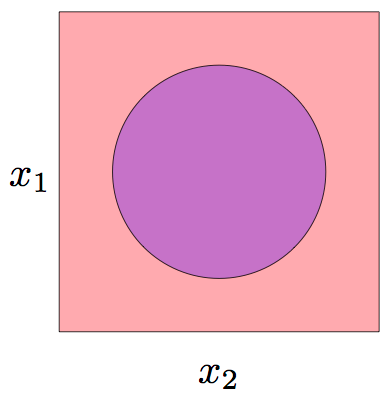
\includegraphics[height=0.5\textheight]{../Figures/features/circularBoundary}
\par\end{center}
\begin{itemize}
\item With identity feature map $\psi(x)=\left(x_{1},x_{2}\right)$ and
linear models, can't separate regions

\pause{}
\item With appropriate featurization $\psi(x)=\left(x_{1},x_{2},x_{1}^{2}+x_{2}^{2}\right)$,
becomes linearly separable . 

\pause{}
\item Video: \url{http://youtu.be/3liCbRZPrZA} 
\end{itemize}
\let\thefootnote\relax\footnotetext{\tiny{From Percy Liang's "Lecture 3" slides from Stanford's CS221, Autumn 2014. }}
\end{frame}
%
\begin{frame}{The Kernel Function}
\begin{itemize}
\item \textbf{Input space}: $\cx$

\pause{}
\item \textbf{Feature space}: $\ch$ (a Hilbert space, i.e. an inner product
space with projections, e.g. $\reals^{d}$)

\pause{}
\item \textbf{Feature map}: $\psi:\cx\to\ch$

\pause{}
\item The \textbf{kernel function} corresponding to $\psi$ is 
\[
k(x,x')=\left\langle \psi(x),\psi(x')\right\rangle ,
\]
where $\left\langle \cdot,\cdot\right\rangle $ is the inner product
associated with $\ch$.
\end{itemize}
\end{frame}
%
\begin{frame}{The Kernel Function: Why do we need this?}
\begin{itemize}
\item \textbf{Feature map}: $\psi:\cx\to\ch$
\item The \textbf{kernel function} corresponding to $\psi$ is 
\[
k(x,x')=\left\langle \psi(x),\psi(x')\right\rangle .
\]
\end{itemize}

\pause{}
\begin{itemize}
\item Why introduce this new notation $k(x,x')$?
\end{itemize}

\pause{}
\begin{itemize}
\item We can often evaluate $k(x,x')$ without explicitly computing $\psi(x)$
and $\psi(x')$.
\end{itemize}

\pause{}
\begin{itemize}
\item For large feature spaces, can be much faster.
\end{itemize}
\end{frame}

%
\begin{frame}{What are the Benefits of Kernelization?}
\begin{enumerate}
\item Computational (when optimizing over $\reals^{n}$ is better than over
$\reals^{d}$)). 

\pause{}
\item Can sometimes avoid any $O(d)$ operations
\begin{itemize}
\item allows access to\textbf{ infinite-dimensional feature spaces}.
\end{itemize}

\pause{}
\item Allows thinking in terms of ``similarity'' rather than features.
\end{enumerate}
\end{frame}
%
\section{The Representer Theorem to Kernelize}
\begin{frame}{The Representer Theorem}
\begin{theorem}
[Representer Theorem] Let 
\[
J(w)=R\left(\|w\|\right)+L\left(\left\langle w,x_{1}\right\rangle ,\ldots,\left\langle w,x_{n}\right\rangle \right),
\]
where
\begin{itemize}
\item $w,x_{1},\ldots,x_{n}\in\ch$ for some Hilbert space $\ch$. (We typically
have $\ch=\reals^{d}.)$
\item $\|\cdot\|$ is the norm corresponding to the inner product of $\ch$.
(i.e. $\|w\|=\sqrt{\left\langle w,w\right\rangle }$) 
\item $R:[0,\infty)\to\reals$ is nondecreasing (\textbf{Regularization
term}), and
\item $L:\reals^{n}\to\reals$ is arbitrary (\textbf{Loss term}).
\end{itemize}
If $J(w)$ has a minimizer, then it \textbf{has a minimizer of the
form} $w^{*}=\sum_{i=1}^{n}\alpha_{i}x_{i}.$\\
{[}If $R$ is strictly increasing, then all minimizers have this form.
(Proof in homework.){]}
\end{theorem}

\end{frame}
%
\begin{frame}{Questions on Representer Theorem}
\begin{itemize}
\item If $J(w)$ is the objective function of the following problems, \\do all the minimizers have the form $w^* = \sum_{i=1}^n\alpha_i x_i$?
\begin{itemize}
\item Lasso regression? 
\item Ridge regression?
\end{itemize}
\end{itemize}
\end{frame}
%
\begin{frame}{Questions on Representer Theorem}
\begin{itemize}
\item If $J(w)$ is the objective function of the following problems, \\do all the minimizers have the form $w^* = \sum_{i=1}^n\alpha_i x_i$?
\begin{itemize}
\item Lasso regression? \textbf{Not Always}
\item Ridge regression? \textbf{All the minimizers have the form.}
\end{itemize}
\item (Copy from Representer Theorem) 
\begin{itemize}
\item $R:[0,\infty)\to\reals$ is nondecreasing of $\|w\|$. If $J(w)$ has a minimizer, then it \textbf{has a minimizer of the
form} $w^{*}=\sum_{i=1}^{n}\alpha_{i}x_{i}.$
\item If $R$ is strictly increasing, then all minimizers have this form.
\end{itemize}
\end{itemize}
\end{frame}
%
\begin{frame}{A Simple Example}
\begin{itemize}
\item Suppose we only have one data point $x_1 = 1, x_2 = 1, y =1$.	
\pause{}
\item Lasso regression: $J(w) = (y-w_1x_1-w_2x_2)^2 + |w_1|+|w_2|$. 
\pause{}
\item Lasso regression is equivalent to (Homework 4):
\begin{align*}
\min_w & \quad J(w) = (y-w_1x_1-w_2x_2)^2 	\\
s.t. & \quad |w_1|+|w_2| \leq r
\end{align*}
\item There is no closed form solution of $r$. But we can still analyze using $r$. All solutions $(w_1, w_2)$ are on the line segment $w_1+w_2 = r, \quad 0\leq w_1,w_2\leq r$. Only the one $(w_1 = r/2, w_2 = r/2)$ is a linear combination of $(x_1,x_2)$.
\pause{}
\item For ridge regression: $J(w) = (y-w_1x_1-w_2x_2)^2 + w_1^2+w_2^2$ \pause{}
\item Solution is $(w_1 = 1/3, w_2 = 1/3)$, which is a linear combination of $(x_1,x_2)$.
\end{itemize}
\end{frame}

\begin{frame}{Representer Theorem (Baby Version)}
  \begin{theorem}[(Baby) Representer Theorem]
    Suppose you have a loss function of the form
    $$J(w) = L(w^T\phi(x_1),\ldots,w^T\phi(x_n)) + R(\|w\|_2)$$
    where
    \begin{itemize}
    \item $w,\phi(x_i)\in\reals^D$.
    \item $L:\reals^n\to\reals$ is an arbitrary function (loss term).
    \item $R:\reals_{\geq 0}\to\reals$ is increasing (regularization term).
    \end{itemize}
    Assume $J$ has at least one minimizer.
    Then $J$ has a minimizer $w^*$ of the form $w^*=\sum_{i=1}^n
    \alpha_i\phi(x_i)$ for some $\alpha\in\reals^n$.  If $R$ is strictly increasing, then all
    minimizers have this form.
  \end{theorem}
\end{frame}


\section{Kernels}
\begin{frame}{Linear Kernel}
 
\begin{itemize}
\item Input space: $\cx=\reals^{d}$
\item Feature space: $\ch=\reals^{d}$, with standard inner product

\pause{}
\item Feature map
\[
\psi(x)=x
\]
\item Kernel: 
\[
k(x,x')=x^{T}x'
\]
\end{itemize}
\end{frame}
%
\begin{frame}{Quadratic Kernel in $\reals^{d}$}
 
\begin{itemize}
\item Input space $\cx=\reals^{d}$
\item Feature space: $\ch=\reals^{D}$, where $D=d+{d \choose 2}\approx d^{2}/2$.
\item Feature map:
\[
\ensuremath{\psi(x)=(x_{1},\ldots,x_{d},x_{1}^{2},\ldots,x_{d}^{2},\sqrt{2}x_{1}x_{2},\ldots,\sqrt{2}x_{i}x_{j},\ldots\sqrt{2}x_{d-1}x_{d})^{T}}
\]


\pause{}
\item Then for $\forall x,x'\in\reals^{d}$
\begin{eqnarray*}
k(x,x') & = & \left\langle \psi(x),\psi(x')\right\rangle \\
\pause & = & \left\langle x,x'\right\rangle +\left\langle x,x'\right\rangle ^{2}
\end{eqnarray*}


\pause{}
\item Computation for inner product with explicit mapping: $O(d^{2})$
\item Computation for implicit kernel calculation: $O(d)$.
\end{itemize}
\let\thefootnote\relax\footnotetext{\tiny{Based on Guillaume Obozinski's Statistical Machine Learning course at Louvain, Feb 2014.}}
\end{frame}
%
\begin{frame}{Polynomial Kernel in $\reals^{d}$}
 
\begin{itemize}
\item Input space $\cx=\reals^{d}$
\item Kernel function:
\[
k(x,x')=\left(1+\left\langle x,x'\right\rangle \right)^{M}
\]


\pause{}
\item Corresponds to a feature map with all monomials up to degree $M$.

\pause{}
\item For any $M$, computing the kernel has same computational cost

\pause{}
\item Cost of explicit inner product computation grows rapidly in $M$.
\end{itemize}
\end{frame}

\section{The RBF Kernel}

\begin{frame}{Radial Basis Function (RBF) / Gaussian Kernel}
 
\begin{itemize}
\item Input space $\cx=\reals^{d}$
\[
k(x,x')=\exp\left(-\frac{\|x-x'\|^{2}}{2\sigma^{2}}\right),
\]
where $\sigma^{2}$ is known as the bandwidth parameter.

\pause{}
\item Does it act like a similarity score?

\pause{}
\item Why ``radial''?

\pause{}
\item Have we departed from our ``inner product of feature vector'' recipe?

\pause{}
\begin{itemize}
\item Yes and no: corresponds to an infinite dimensional feature vector

\pause{}
\end{itemize}
\item Probably the most common nonlinear kernel.
\end{itemize}
\end{frame}
%
\begin{frame}{The Infinite Dimensional Feature Vector for RBF}
\begin{itemize}
\item Consider RBF kernel (1-dim): $k(x,x')=\exp\left(-\left(x-x'\right)^{2}/2\right)$
\item We claim that $\psi:\reals\to\ell_{2}$, defined by 
\[
\left[\psi(x)\right]_{j}=\frac{1}{\sqrt{j!}}e^{-x^{2}/2}x^{j}
\]
 gives the \textbf{``infinite-dimensional feature vector'' corresponding
to RBF kernel}.

\pause{}
\item Is this mapping even well-defined? Is $\psi(x)$ even an element of
$\ell_{2}$?

\pause{}
\item Yes: 
\[
\sum_{j=0}^{\infty}\frac{1}{j!}e^{-x^{2}}x^{2j}=e^{-x^{2}}\sum_{j=0}^{\infty}\frac{\left(x^{2}\right)^{j}}{j!}=1<\infty
\]
. 
\end{itemize}
\end{frame}
%
\section{When is $k(x,x')$ a kernel function? (Mercer's Theorem)}
\begin{frame}{How to Get Kernels?}
\begin{enumerate}
\item Explicitly construct $\psi(x):\cx\to\reals^{d}$ and define $k(x,x')=\psi(x)^{T}\psi(x')$.

\pause{}
\item Directly define the kernel function $k(x,x')$, and verify it corresponds
to $\left\langle \psi(x),\psi(x')\right\rangle $ for some $\psi$.

\pause{}

\end{enumerate}
There are many theorems to help us with the second approach

\end{frame}

\begin{frame}{Positive Semidefinite Matrices}
\begin{definition}
A real, symmetric matrix $M\in\reals^{n\times n}$ is \textbf{positive
semidefinite (psd)} if for any $x\in\reals^{n}$, 
\[
x^{T}Mx\ge0.
\]

\pause{}

\end{definition}

\begin{theorem}
The following conditions are each necessary and sufficient for a symmetric
matrix $M$ to be positive semidefinite:
\begin{itemize}
\item $M$ has can be factorized as $M=R^{T}R$, for some matrix $R$.
\item All eigenvalues of $M$ are greater than or equal to $0$.
\end{itemize}
\end{theorem}

\end{frame}
%
\begin{frame}{Positive Semidefinite Function}
\begin{definition}
A symmetric kernel function $k:\cx\times\cx\to\reals$ is \textbf{positive
semidefinite (psd)} if for any finite set $\left\{ x_{1},\ldots,x_{n}\right\} \in\cx$,
the kernel matrix on this set 
\[
K=\begin{pmatrix}k(x_{i},x_{j})\end{pmatrix}_{i,j}=\begin{pmatrix}k(x_{1},x_{1}) & \cdots & k(x_{1},x_{n})\\
\vdots & \ddots & \cdots\\
k(x_{n},x_{1}) & \cdots & k(x_{n},x_{n})
\end{pmatrix}
\]
is a positive semidefinite matrix.
\end{definition}

\end{frame}

\begin{frame}{Mercer's Theorem}
\begin{theorem}
A symmetric function $k(x,x')$ can be expressed as an inner product
\[
k(x,x')=\left\langle \psi(x),\psi(x')\right\rangle 
\]
for some $\psi$ if and only if $k(x,x')$ is \textbf{positive semidefinite.}
\end{theorem}

\end{frame}
%
\begin{frame}{Generating New Kernels from Old}
\begin{itemize}
\item Suppose $k,k_{1},k_{2}:\cx\times\cx\to\reals$ are psd kernels. Then
so are the following:
\begin{eqnarray*}
k_{\mbox{new}}(x,x') & = & k_{1}(x,x')+k_{2}(x,x')\\
k_{\mbox{new}}(x,x') & = & \alpha k(x,x')\\
k_{\mbox{new}}(x,x') & = & f(x)f(x')\mbox{ for any function \ensuremath{f(\cdot)}}\\
k_{\mbox{new}}(x,x') & = & k_{1}(x,x')k_{2}(x,x')
\end{eqnarray*}
\item See Appendix for details.
\item Lots more theorems to help you construct new kernels from old...
\end{itemize}
\end{frame}
%

\appendix

\section{Details on New Kernels from Old {[}Optional{]}}
\begin{frame}{Additive Closure}
\begin{itemize}
\item Suppose $k_{1}$ and $k_{2}$ are psd kernels with feature maps $\phi_{1}$
and $\phi_{2}$, respectively.
\item Then 
\[
k_{1}(x,x')+k_{2}(x,x')
\]
is a psd kernel.

\pause{}
\item Proof: Concatenate the feature vectors to get 
\[
\phi(x)=\left(\phi_{1}(x),\phi_{2}(x)\right).
\]
Then $\phi$ is a feature map for $k_{1}+k_{2}$. 
\end{itemize}
\end{frame}
%
\begin{frame}{Closure under Positive Scaling}
\begin{itemize}
\item Suppose $k$ is a psd kernel with feature maps $\phi$.
\item Then for any $\alpha>0$, 
\[
\alpha k
\]
is a psd kernel.

\pause{}
\item Proof: Note that 
\[
\phi(x)=\sqrt{\alpha}\phi(x)
\]
 is a feature map for $\alpha k$.
\end{itemize}
\end{frame}
%
\begin{frame}{Scalar Function Gives a Kernel}
\begin{itemize}
\item For any function $f(x)$, 
\[
k(x,x')=f(x)f(x')
\]
is a kernel.

\pause{}
\item Proof: Let $f(x)$ be the feature mapping. (It maps into a 1-dimensional
feature space.)
\[
\left\langle f(x),f(x')\right\rangle =f(x)f(x')=k(x,x').
\]
\end{itemize}
\end{frame}
%
\begin{frame}{Closure under Hadamard Products}
\begin{itemize}
\item Suppose $k_{1}$ and $k_{2}$ are psd kernels with feature maps $\phi_{1}$
and $\phi_{2}$, respectively.
\item Then 
\[
k_{1}(x,x')k_{2}(x,x')
\]
is a psd kernel.

\pause{}
\item Proof: Take the outer product of the feature vectors: 
\[
\phi(x)=\phi_{1}(x)\left[\phi_{2}(x)\right]^{T}.
\]
Note that $\phi(x)$ is a matrix.
\item Continued...
\end{itemize}
\end{frame}
%
\begin{frame}{Closure under Hadamard Products}
\begin{itemize}
\item Then
\begin{eqnarray*}
\left\langle \phi(x),\phi(x')\right\rangle  & = & \sum_{i,j}\phi(x)\phi(x')\\
 & = & \sum_{i,j}\left[\phi_{1}(x)\left[\phi_{2}(x)\right]^{T}\right]_{ij}\left[\phi_{1}(x')\left[\phi_{2}(x')\right]^{T}\right]_{ij}\\
 & = & \sum_{i,j}\left[\phi_{1}(x)\right]_{i}\left[\phi_{2}(x)\right]_{j}\left[\phi_{1}(x')\right]_{i}\left[\phi_{2}(x')\right]_{j}\\
 & = & \left(\sum_{i}\left[\phi_{1}(x)\right]_{i}\left[\phi_{1}(x')\right]_{i}\right)\left(\sum_{j}\left[\phi_{2}(x)\right]_{j}\left[\phi_{2}(x')\right]_{j}\right)\\
 & = & k_{1}(x,x')k_{2}(x,x')
\end{eqnarray*}
\end{itemize}
\end{frame}
\section{Questions on Kernel Methods}
\begin{frame}
\begin{enumerate}
\item Fix $n>0$.  For $x,y\in\{1,2,\ldots,n\}$ define
  $k(x,y)=\min(x,y)$.  Give an explicit feature map
  $\phi:\{1,2,\ldots,n\}$ to $\reals^D$ (for some $D$) such that
  $k(x,y)=\phi(x)^T\phi(y)$.	
 \item Show that $k(x,y) = (x^Ty)^4$ is a positive semidefinite kernel
  on $\reals^d\times\reals^d$.
  \item Let $A\in\reals^{d\times d}$ be a positive semidefinite matrix.
  Prove that $k(x,y)= x^TAy$ is a positive semidefinite kernel.

\end{enumerate}	
\end{frame}
\begin{frame}
\begin{enumerate}
\item Fix $n>0$.  For $x,y\in\{1,2,\ldots,n\}$ define
  $k(x,y)=\min(x,y)$.  Give an explicit feature map
  $\phi:\{1,2,\ldots,n\}$ to $\reals^D$ (for some $D$) such that
  $k(x,y)=\phi(x)^T\phi(y)$.
  \item[]
  \textbf{Solution:}\\
   Define $\phi(x) = (\mathds{1}(x\geq 1),\mathds{1}(x\geq
  2),\ldots,\mathds{1}(x\geq n))$.  Then $\phi(x)^T\phi(y)=\min(x,y)$.
  \item Show that $k(x,y) = (x^Ty)^4$ is a positive semidefinite kernel
  on $\reals^d\times\reals^d$.
\item[]
\textbf{Solution: } \\
 $k_1(x,y)=x^Ty$ is a psd kernel, since $x^Ty$ is an inner
  product on $\reals^d$.  Using the product rule for psd kernels, we see
  that
  $$k(x,y)=k_1(x,y)k_1(x,y)k_1(x,y)k_1(x,y) = k_1(x,y)^4$$
  is psd as well.
  \end{enumerate}
	
\end{frame}
\begin{frame}
\begin{enumerate}
 \item Let $A\in\reals^{d\times d}$ be a positive semidefinite matrix.
  Prove that $k(x,y)= x^TAy$ is a positive semidefinite kernel.
\item[]\textbf{Solution:}\\
Fix $x_1,\ldots,x_n\in\reals^d$ and let $X$ denote the matrix
  that has $x_i^T$ as its $i$th row.  Then note that
  $(XAX^T)_{ij} = x_i^TAx_j = k(x_i,x_j)$.  Thus we are done if we can
  show $XAX^T$ is positive semidefinite.  But note that, for any $\alpha\in\reals^n$,
  $$\alpha^TXAX^T\alpha = (X^T\alpha)^T A (X^T\alpha) \geq 0,$$
  since $A$ is positive semidefinite.	
\end{enumerate}	
\end{frame}
\begin{frame}
\begin{enumerate}
\item Suppose you are given an training set of distinct points
  $x_1,x_2,\ldots,x_n\in\reals^n$ and labels
  $y_1,\ldots,y_n\in\{-1,+1\}$.  Show that by properly selecting
  $\sigma$ you can achieve perfect $0-1$ loss on the training data
  using a linear decision function and the RBF kernel.
\item Consider the standard (unregularized) linear regression problem
  where we minimize $L(w)=\|Xw-y\|_2^2$ for some $X\in\reals^{n\times m}$ and
  $y\in\reals^n$.  Assume $m > n$.
  \begin{enumerate}
  \item Let $w^*$ be one minimizer of the loss function $L$ above.
    Give an infinite set of minimizers of the loss function.
  \item What property defines the minimizer given by the representer
    theorem (in terms of $X$)?
  \end{enumerate}
	
\end{enumerate}
\end{frame}
\begin{frame}
\begin{enumerate}
\item Suppose you are given an training set of distinct points
  $x_1,x_2,\ldots,x_n\in\reals^n$ and labels
  $y_1,\ldots,y_n\in\{-1,+1\}$.  Show that by properly selecting
  $\sigma$ you can achieve perfect $0-1$ loss on the training data
  using a linear decision function and the RBF kernel.
\item[]\textbf{Solution: }\\
 By selecting $\sigma$ sufficiently small (say, much
  smaller than $\min_{i\neq j}\|x_i-x_j\|_2$) we can use
  $\alpha_i=y_i$ and get very pointy spikes at each data point. Kernelized prediction function will be:
  \begin{align*}
  f(x) &= \sum_{i=1}^n y_i \exp(-\|x-x_i\|_2^2/\sigma^2),\\
  f(x_j) & = y_j + \sum_{i\neq j} y_i \exp(-\|x_j-x_i\|^2_2/\sigma^2) , 
  \end{align*}
  where $|y_j|>> |\sum_{i\neq j} y_i \exp(-\|x_j-x_i\|^2_2/\sigma^2)|$.
  \item[][Note:
    This is not possible if any repeated points have different labels,
    which is not unusual in real data.]	
\end{enumerate}	
\end{frame}
\begin{frame}
\begin{enumerate}
\item  Consider the standard (unregularized) linear regression problem
  where we minimize $L(w)=\|Xw-y\|_2^2$ for some $X\in\reals^{n\times m}$ and
  $y\in\reals^n$.  Assume $m > n$.
  \begin{enumerate}
  \item Let $w^*$ be one minimizer of the loss function $L$ above.
    Give an infinite set of minimizers of the loss function.
  \item What property defines the minimizer given by the representer
    theorem (in terms of $X$)?
    \end{enumerate}
 \item[]\textbf{Solution:}\\
  \begin{enumerate}
  \item $\{w^* + v\mid v\in\text{Null}(X)\}$.  Using the standard inner
    product on $\reals^n$, we can also write $\text{Null}(X)$ as the set of all
    vectors orthogonal to the row space of $X$.x
  \item $w^*$ lies in the row space of $X$.
	\end{enumerate}
\end{enumerate}	
\end{frame}

\end{document}
